%%%%%%%%%%%%%%%%%%%%%%%%%%%%%%%%%%%%%%%%%
% Arsclassica Article
% LaTeX Template
% Version 1.1 (1/8/17)
%
% This template has been downloaded from:
% http://www.LaTeXTemplates.com
%
% Original author:
% Lorenzo Pantieri (http://www.lorenzopantieri.net) with extensive modifications by:
% Vel (vel@latextemplates.com)
%
% License:
% CC BY-NC-SA 3.0 (http://creativecommons.org/licenses/by-nc-sa/3.0/)
%
%%%%%%%%%%%%%%%%%%%%%%%%%%%%%%%%%%%%%%%%%

%----------------------------------------------------------------------------------------
%	PACKAGES AND OTHER DOCUMENT CONFIGURATIONS
%----------------------------------------------------------------------------------------

\documentclass[
12pt, % Main document font size
a4paper, % Paper type, use 'letterpaper' for US Letter paper
oneside, % One page layout (no page indentation)
%twoside, % Two page layout (page indentation for binding and different headers)
headinclude,footinclude, % Extra spacing for the header and footer
BCOR5mm, % Binding correction
]{scrartcl}

%%%%%%%%%%%%%%%%%%%%%%%%%%%%%%%%%%%%%%%%%
% Arsclassica Article
% Structure Specification File
%
% This file has been downloaded from:
% http://www.LaTeXTemplates.com
%
% Original author:
% Lorenzo Pantieri (http://www.lorenzopantieri.net) with extensive modifications by:
% Vel (vel@latextemplates.com)
%
% License:
% CC BY-NC-SA 3.0 (http://creativecommons.org/licenses/by-nc-sa/3.0/)
%
%%%%%%%%%%%%%%%%%%%%%%%%%%%%%%%%%%%%%%%%%

%----------------------------------------------------------------------------------------
%	REQUIRED PACKAGES
%----------------------------------------------------------------------------------------

\usepackage[
nochapters, % Turn off chapters since this is an article        
beramono, % Use the Bera Mono font for monospaced text (\texttt)
eulermath,% Use the Euler font for mathematics
pdfspacing, % Makes use of pdftex’ letter spacing capabilities via the microtype package
dottedtoc % Dotted lines leading to the page numbers in the table of contents
]{classicthesis} % The layout is based on the Classic Thesis style

\usepackage{arsclassica} % Modifies the Classic Thesis package

\usepackage[T1]{fontenc} % Use 8-bit encoding that has 256 glyphs

\usepackage[utf8]{inputenc} % Required for including letters with accents

\usepackage{graphicx} % Required for including images
\graphicspath{{Figures/}} % Set the default folder for images

\usepackage{enumitem} % Required for manipulating the whitespace between and within lists

\usepackage{lipsum} % Used for inserting dummy 'Lorem ipsum' text into the template

\usepackage{subfig} % Required for creating figures with multiple parts (subfigures)

\usepackage{amsmath,amssymb,amsthm} % For including math equations, theorems, symbols, etc

\usepackage{varioref} % More descriptive referencing

\usepackage{listings}
%----------------------------------------------------------------------------------------
%	THEOREM STYLES
%---------------------------------------------------------------------------------------

\theoremstyle{definition} % Define theorem styles here based on the definition style (used for definitions and examples)
\newtheorem{definition}{Definition}

\theoremstyle{plain} % Define theorem styles here based on the plain style (used for theorems, lemmas, propositions)
\newtheorem{theorem}{Theorem}

\theoremstyle{remark} % Define theorem styles here based on the remark style (used for remarks and notes)

%----------------------------------------------------------------------------------------
%	HYPERLINKS
%---------------------------------------------------------------------------------------

\hypersetup{
%draft, % Uncomment to remove all links (useful for printing in black and white)
colorlinks=true, breaklinks=true, bookmarks=true,bookmarksnumbered,
urlcolor=webbrown, linkcolor=RoyalBlue, citecolor=webgreen, % Link colors
pdftitle={}, % PDF title
pdfauthor={\textcopyright}, % PDF Author
pdfsubject={}, % PDF Subject
pdfkeywords={}, % PDF Keywords
pdfcreator={pdfLaTeX}, % PDF Creator
pdfproducer={LaTeX with hyperref and ClassicThesis} % PDF producer
} % Include the structure.tex file which specified the document structure and layout

\hyphenation{Fortran hy-phen-ation} % Specify custom hyphenation points in words with dashes where you would like hyphenation to occur, or alternatively, don't put any dashes in a word to stop hyphenation altogether

%----------------------------------------------------------------------------------------
%	TITLE AND AUTHOR(S)
%----------------------------------------------------------------------------------------

\title{\normalfont\spacedallcaps{ERG3020 Report}} % The article title

%\subtitle{Subtitle} % Uncomment to display a subtitle

\author{\spacedlowsmallcaps{Zhuoyu Li\& Bokai Xu\& Xiyan Luo}} % The article author(s) - author affiliations need to be specified in the AUTHOR AFFILIATIONS block

\date{2021.5.5} % An optional date to appear under the author(s)

%----------------------------------------------------------------------------------------

\begin{document}

%----------------------------------------------------------------------------------------
%	HEADERS
%----------------------------------------------------------------------------------------

\renewcommand{\sectionmark}[1]{\markright{\spacedlowsmallcaps{#1}}} % The header for all pages (oneside) or for even pages (twoside)
%\renewcommand{\subsectionmark}[1]{\markright{\thesubsection~#1}} % Uncomment when using the twoside option - this modifies the header on odd pages
\lehead{\mbox{\llap{\small\thepage\kern1em\color{halfgray} \vline}\color{halfgray}\hspace{0.5em}\rightmark\hfil}} % The header style

\pagestyle{scrheadings} % Enable the headers specified in this block

%----------------------------------------------------------------------------------------
%	TABLE OF CONTENTS & LISTS OF FIGURES AND TABLES
%----------------------------------------------------------------------------------------

\maketitle % Print the title/author/date block

\setcounter{tocdepth}{2} % Set the depth of the table of contents to show sections and subsections only

\tableofcontents % Print the table of contents

% \listoffigures % Print the list of figures

% \listoftables % Print the list of tables

%----------------------------------------------------------------------------------------
%	ABSTRACT
%----------------------------------------------------------------------------------------

\section*{Abstract} % This section will not appear in the table of contents due to the star (\section*)

This project is a demo of social network comment section with a special algorithm on the sorting and the presentation of comments. We aim at find and tell the truth so that we combine Natural Language Processing and Markov Networks to make a demo of social network comment section and we hope that a better social network comment section can be guaranteed.



%----------------------------------------------------------------------------------------
%	AUTHOR AFFILIATIONS
%----------------------------------------------------------------------------------------

\let\thefootnote\relax\footnotetext{* \textit{School of Data Science, The Chinese University of Hong Kong, Shenzhen, China}}



%----------------------------------------------------------------------------------------

\newpage % Start the article content on the second page, remove this if you have a longer abstract that goes onto the second page

%----------------------------------------------------------------------------------------
%	INTRODUCTION
%----------------------------------------------------------------------------------------
\section{Introduction}
\subsection{The Properties of Markov Network and the Origin of Our Idea}
Markov Network is an undirected graphical model for representing dependencies between random variables.

A Markov network can be represented by an undirected graph $G = (V,E)$ where the nodes in $V$ represent random variables
and edges in $E$ represent dependency relationships.

Let us consider $X$, a kind of assignment of values to the variables in a Markov Network. We call $C$ the set of maximal
cliques in the network and assign a factor $\psi_c$ to each clique $c \in C$. The probability $P(X)$ is,

\begin{equation}
    P(X=x)=\frac{1}{Z}\prod_k\phi_k(x_{(k)})
\end{equation}

We know that Markov Network can be used to represent a system, where this system is in general form, because the random
variables in $V$ can be either numerical or categorical.

If we want to represent a world in the form of Markov Network, we can consider binary case, for example, if Tom lied, we
can assign \textbf{True} to the random variable \textbf{lie(Tom)}. So each random variable in our desired network can only take one of
the two binary values \textbf{\{True, False\}}.

The world above is an assignment of values of $V$.

We are continuously thinking about the way to infer the truth of the event. PageRank algorithm by Jimmy Page gave us the
confidence to utilize graph theory to solve the truth of an event. We tried Pagerank Algorithm to infer the truth of an
event by assigning the relationship \textbf{\{Entailment, Contradiction, Independence\}} between any pairs of comments on
the social network. Then we construct a directed graph of this set of comments. Each comment will post its importance to
the comment that it entails, and we can construct a transition matrix, and then calculate $A^500$ or above, until the matrix
converges. Then we can find the stationary point. Then we can rank the comments according to their PageRank value. In this process,
we observe the specfic property of graph. However, this algorithm may not work very well in practice, because its time complexity is $O(n!)$. 
Now we focus on the combination of graph and First Oerder Logic. 

We find that undirectional graph may perform better than directional graph. Because the computer cannot really understand what you mean at a extremely high
precision, and the sentences generated by users may not entail each other by our definition. So, to use First Order Logic and build an undirectional graph may be better than PageRank algorithm when we analyse the comments by netizens.







\section{Knowledges used in the Project}
\subsection{Natural Language Processing}
Natural language processing (NLP) is a field concerned with the interactions between computers and human language, in particular how to program computers to process and analyze large amounts of natural language data. The result is a computer capable of "understanding" the contents of documents, including the contextual nuances of the language within them \cite{enwiki:1020063620}.

We have to deal with the natural language records so that we have to choose some NLP algorithms. The most important part is to do text segmentations, transfer the texts into first order logic and atomic sentences to match the requirements of the Markov Logic Network.

\subsection{Markov Logic Networks}
The markov networks model used in this project comes from the article written by Richardson and Domingos in 2006 \cite{richardson2006markov}. The below statements in this subsection are from the article.

A Markov network (also known as Markov random field) is a model for the joint distribution of a set of variables $X = (X_1,X_2,\cdots,X_n) \in X$. The joint distribution represented by a Markov network is given by
\begin{equation}
    P(X=x)=\frac{1}{Z}\prod_k\phi_k(x_{(k)})
\end{equation}
where $x_{(k)}$ is the state of the $k$th clique (i.e., the state of the variables that appear in that clique). $Z$, known as the \textit{partition function}, is given by $Z=\sum_{x\in X}\prod_k\phi_k(x_{(k)})$.
\begin{definition}[Markov logic network]
    A Markov logic network L is a set of pairs $(F_i, w_i)$, where $F_i$ is a formula in first-order logic and $w_i$ is a real number. Together with a finite set of constants $C = {c_1,c_2,\cdots,c_{|C|}}$, it defines a Markov network $M_{L,C}$ (Equations 1 and 2) as follows:
\end{definition}

\begin{enumerate}[noitemsep]
    \item \textit{$M_{L,C}$ contains one binary node for each possible grounding of each predicate appearing in $L$. The value of the node is $1$ if the ground atom is true, and $0$ otherwise.}
    \item \textit{$M_{L,C}$ contains one feature for each possible grounding ofeach formula $F_i$ in $L$. The value ofthis feature is $1$ if the ground formula is true, and $0$ otherwise. The weight ofthe feature is the wi associated with $F_i$ in $L$.}
\end{enumerate}

All the formulas and the constants in the Markov Logic Networks have to meet the $3$ assumptions below:

\begin{enumerate}[noitemsep]
    \item \textbf{Unique names.} \textit{Different constants refer to different objects.}
    \item \textbf{Domain closure.} \textit{The only objects in the domain are those representable using the constant and function symbols in $(L,C)$}
    \item \textbf{Known functions.} \textit{For each function appearing in $L$, the value of the function applied to every possible tuple of arguments is known, and is a element of $C$.}
\end{enumerate}



\section{Packages used in the Project}
\subsection{Natural Language Processing}
The NLP package used in this project is \textbf{AllenNLP} \cite{Gardner2017AllenNLP}. We use the methods of AllenNLP to do text segmentations, transfer the texts into first order logic and atomic sentences so that we can match the requirements from the Markov Logic Network.

\subsection{Markov Logic Networks}
\textbf{Pracmln} is a toolbox for statistical relational learning and reasoning and as such also includes tools for standard graphical models \cite{pracmln}. We use this package to build the markov logic networks and give the results.
\subsection{Flask}
\textbf{Flask} is a micro web framework written in Python 
\cite{grinberg2018flask}. We use \textbf{Flask} to show the demo of social network comments section. Here is a figure of the demo website:
\begin{figure}[tb]
    \centering 
    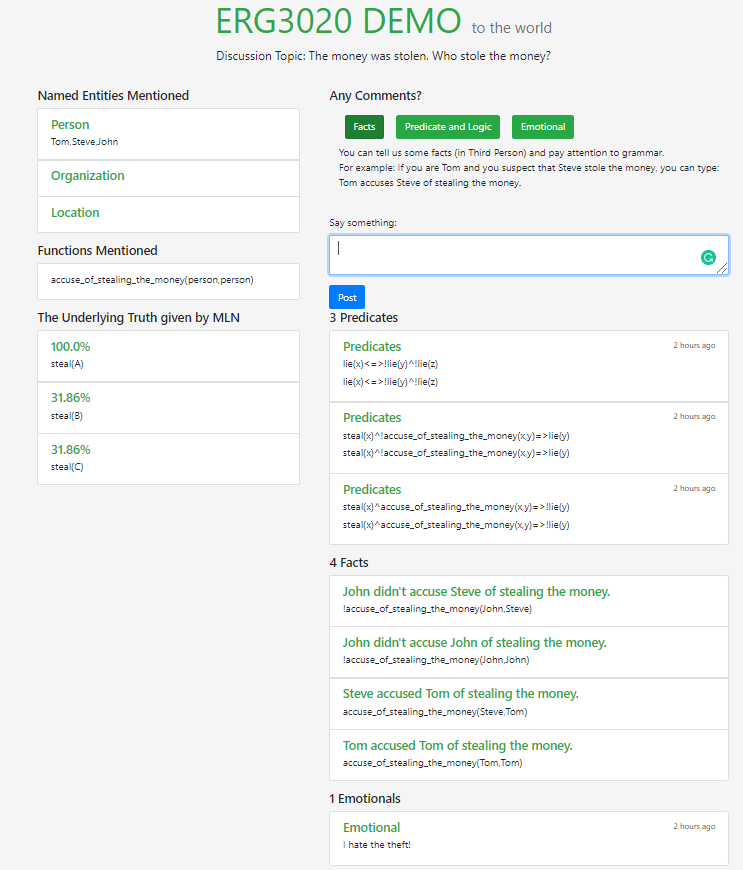
\includegraphics[width=\columnwidth]{Flask.png} 
    \caption[An Screenshot of the website]{An Screenshot of the website} % The text in the square bracket is the caption for the list of figures while the text in the curly brackets is the figure caption
    \end{figure}
From the website, we can find that:

\section{Introduction}

A statement requiring citation.

\lipsum[1-3] % Dummy text

Some mathematics in the text: $\cos\pi=-1$ and $\alpha$.
 
%----------------------------------------------------------------------------------------
%	METHODS
%----------------------------------------------------------------------------------------

\section{Methods}

\lipsum[5] % Dummy text

\begin{enumerate}[noitemsep] % [noitemsep] removes whitespace between the items for a compact look
\item First item in a list
\item Second item in a list
\item Third item in a list
\end{enumerate}

%------------------------------------------------

\subsection{Paragraphs}

\lipsum[6] % Dummy text

\paragraph{Paragraph Description} \lipsum[7] % Dummy text

\paragraph{Different Paragraph Description} \lipsum[8] % Dummy text

%------------------------------------------------

\subsection{Math}

\lipsum[4] % Dummy text

\begin{equation}
\cos^3 \theta =\frac{1}{4}\cos\theta+\frac{3}{4}\cos 3\theta
\label{eq:refname2}
\end{equation}

\lipsum[5] % Dummy text

\begin{definition}[Gauss] 
To a mathematician it is obvious that
$\int_{-\infty}^{+\infty}
e^{-x^2}\,dx=\sqrt{\pi}$. 
\end{definition} 

\begin{theorem}[Pythagoras]
The square of the hypotenuse (the side opposite the right angle) is equal to the sum of the squares of the other two sides.
\end{theorem}

\begin{proof} 
We have that $\log(1)^2 = 2\log(1)$.
But we also have that $\log(-1)^2=\log(1)=0$.
Then $2\log(-1)=0$, from which the proof.
\end{proof}

%----------------------------------------------------------------------------------------
%	RESULTS AND DISCUSSION
%----------------------------------------------------------------------------------------

\section{Results and Discussion}

Reference to Figure~\vref{fig:gallery}. % The \vref command specifies the location of the reference

\begin{figure}[tb]
\centering 
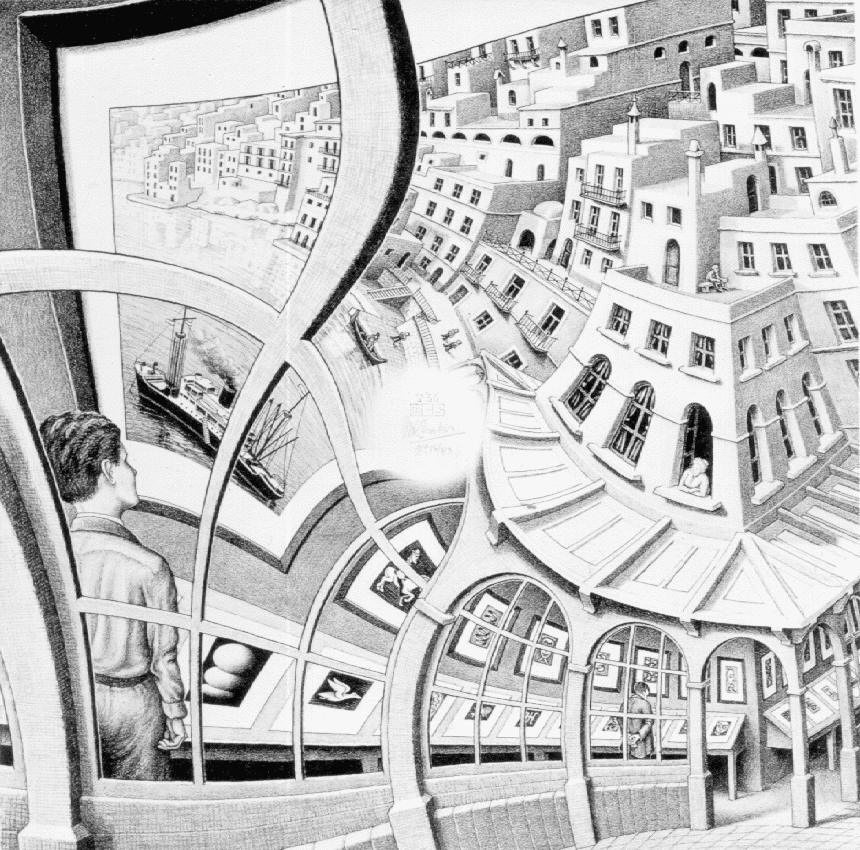
\includegraphics[width=0.5\columnwidth]{GalleriaStampe} 
\caption[An example of a floating figure]{An example of a floating figure (a reproduction from the \emph{Gallery of prints}, M.~Escher,\index{Escher, M.~C.} from \url{http://www.mcescher.com/}).} % The text in the square bracket is the caption for the list of figures while the text in the curly brackets is the figure caption
\label{fig:gallery} 
\end{figure}

\lipsum[10] % Dummy text

%------------------------------------------------

\subsection{Subsection}

\lipsum[11] % Dummy text

\subsubsection{Subsubsection}

\lipsum[12] % Dummy text

\begin{description}
\item[Word] Definition
\item[Concept] Explanation
\item[Idea] Text
\end{description}

\lipsum[12] % Dummy text

\begin{itemize}[noitemsep] % [noitemsep] removes whitespace between the items for a compact look
\item First item in a list
\item Second item in a list
\item Third item in a list
\end{itemize}

\subsubsection{Table}

\lipsum[13] % Dummy text

\begin{table}[hbt]
\caption{Table of Grades}
\centering
\begin{tabular}{llr}
\toprule
\multicolumn{2}{c}{Name} \\
\cmidrule(r){1-2}
First name & Last Name & Grade \\
\midrule
John & Doe & $7.5$ \\
Richard & Miles & $2$ \\
\bottomrule
\end{tabular}
\label{tab:label}
\end{table}

Reference to Table~\vref{tab:label}. % The \vref command specifies the location of the reference

%------------------------------------------------

\subsection{Figure Composed of Subfigures}

Reference the figure composed of multiple subfigures as Figure~\vref{fig:esempio}. Reference one of the subfigures as Figure~\vref{fig:ipsum}. % The \vref command specifies the location of the reference

\lipsum[15-18] % Dummy text

\begin{figure}[tb]
\centering
\subfloat[A city market.]{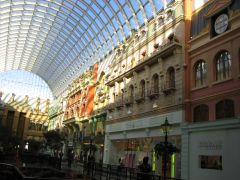
\includegraphics[width=.45\columnwidth]{Lorem}} \quad
\subfloat[Forest landscape.]{
\includegraphics[width=.45\columnwidth]{Ipsum}\label{fig:ipsum}} \\
\subfloat[Mountain landscape.]{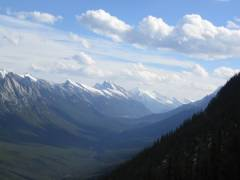
\includegraphics[width=.45\columnwidth]{Dolor}} \quad
\subfloat[A tile decoration.]{
\includegraphics[width=.45\columnwidth]{Sit}}
\caption[A number of pictures.]{A number of pictures with no common theme.} % The text in the square bracket is the caption for the list of figures while the text in the curly brackets is the figure caption
\label{fig:esempio}
\end{figure}

%----------------------------------------------------------------------------------------
%	BIBLIOGRAPHY
%----------------------------------------------------------------------------------------

\renewcommand{\refname}{\spacedlowsmallcaps{References}} % For modifying the bibliography heading


\clearpage
\bibliographystyle{unsrt}

\bibliography{references.bib} % The file containing the bibliography

%----------------------------------------------------------------------------------------
\clearpage
\appendix
\section{A guidence to running code}
First we have to make sure the working director of the ternimal is the code folder. Then we type the below codes:
\begin{lstlisting}
    pip install -r requirements.txt
\end{lstlisting}
Then we can find that all the requirements are installed. The next steps are to run the flask app. 
\begin{lstlisting}
    $env:FLASK_APP = "sayhello"
\end{lstlisting}
And then
\begin{lstlisting}
    flask run --host 127.0.0.1 -p 80
\end{lstlisting}
Therefore, the flask app is run and we can see the website.
\end{document}
